\documentclass{article}
\usepackage{graphicx}
\usepackage{natbib,mybigpackage}
\usepackage{algorithm}
\usepackage{algorithmic}
\usepackage{listings}

\graphicspath{ {} }
\def\xbf{\mathbf{x}}
\def\zbf{\mathbf{z}}
\def\xibf{\mathbf{\xi}}


\title{\textbf{\LARGE Report}\\
\Large Assignment:11\\
\Large{Divyae Vats}\\
\large Roll No. : 140123049}
\date{April 26th, 2016}
\begin{document}
\maketitle
\textbf{\large Question 1(a):}
The Code to implement this Question is as follows:\\

\noindent{R Code}

\lstset {language=R}


\begin{lstlisting}

for(i in 1:25){
	p=NULL;
	res <- 0;
	num=i;
	for(j in 1:5){
		p[j]=num%%2;
		num=num%/%2;
	}
	for(k in 1:5){
		res=res+p[k]*2^(-k);
	}
		cat(res, " ");
}


\end{lstlisting}

The Output of this code gives:\\~\\

0.5  , 0.25  , 0.75  , 0.125  , 0.625  , 0.375  , 0.875  , 0.0625  , 0.5625  , 0.3125  , 0.8125  , 0.1875  , 0.6875  , 0.4375  , 0.9375  , 0.03125  , 0.53125  , 0.28125  , 0.78125  , 0.15625  , 0.65625  , 0.40625  , 0.90625  , 0.09375  , 0.59375.\\~\\~\\
\textbf{\large Question 1(b):}
The Code to implement this Question is as follows:\\

\noindent{R Code}

\lstset {language=R}


\begin{lstlisting}

seq=NULL;
for(i in 1:1000){
	p=NULL;
	res <- 0;
	num=i;
	for(j in 1:11){
		p[j]=num%%2;
		num=num%/%2;
	}
	for(k in 1:11){
		res=res+p[k]*2^(-k);
	}
	seq[i]=res;
}
#Making 2-D pairs.
seq2=NULL;
for(s in 1:999){
	seq2[s]=seq[s+1];
}
#Finding the overlapping values and plotting.

overl1=NULL;
overl2=NULL;
m <- 0;
for(q in 2:999){
	cor1 <- seq[q];
	cor2 <- seq2[q];
	for(r in 2:q-1){
		n1=seq[r];
		n2=seq2[r];
		if((cor1==n1) & (cor2==n2)){
			m=m+1;
			overl1[m]=cor1;
			overl2[m]=cor2;
			break;
		}
	}
}
pk=c(0,1);
plot(overl1,overl2, xlim=pk, ylim=pk);


\end{lstlisting}


\begin{center}
	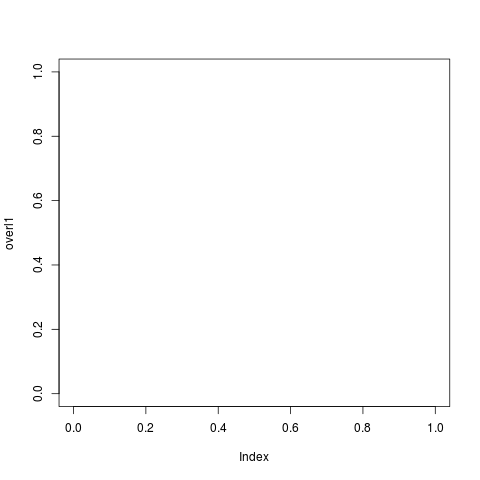
\includegraphics{Question1_2.png}
\end{center}

We observe that there are no values in the plot which shows that none of the sequence of values overlaps with each other.\\

\newpage

\textbf{\large Question 1(c):}
The Code to implement this Question is as follows:\\

\noindent{R Code}

\lstset {language=R}


\begin{lstlisting}

seq=NULL;
for(i in 1:101){
	p=NULL;
	res <- 0;
	num=i;
	for(j in 1:8){
		p[j]=num%%2;
		num=num%/%2;
	}
	for(k in 1:8){
		res=res+p[k]*2^(-k);
	}
	seq[i]=res;
}
#Making 2-D pairs.
seq2=NULL;
for(s in 1:100){
	seq2[s]=seq[s+1];
}
length(seq) <- 100;

pk=c(0,1);
plot(seq,seq2, xlim=pk, ylim=pk);


\end{lstlisting}


\begin{center}
	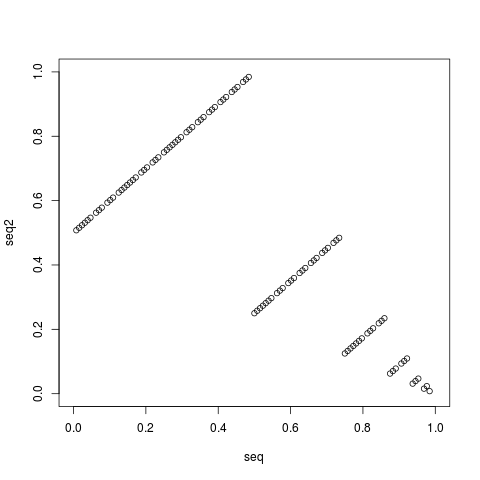
\includegraphics{Question1_3.png}
\end{center}

\newpage
\textbf{\large Question 1(d):}
The Code to implement this Question is as follows:\\

\noindent{R Code}

\lstset {language=R}


\begin{lstlisting}

seq=NULL;
for(i in 1:100001){
	p=NULL;
	res <- 0;
	num=i;
	for(j in 1:18){
		p[j]=num%%2;
		num=num%/%2;
	}
	for(k in 1:18){
		res=res+p[k]*2^(-k);
	}
	seq[i]=res;
}
#Making 2-D pairs.
seq2=NULL;
for(s in 1:100000){
	seq2[s]=seq[s+1];
}
length(seq) <- 100000;

pk=c(0,1);
plot(seq,seq2, xlim=pk, ylim=pk);


\end{lstlisting}


\begin{center}
	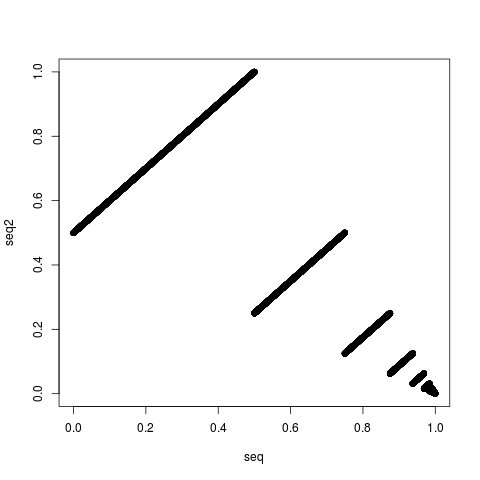
\includegraphics{Question1_4.png}
\end{center}

\newpage
\textbf{\large Question 1(e):}
The Code to implement this Question is as follows:\\

\noindent{R Code}

\lstset {language=R}


\begin{lstlisting}

a <- 1229;
b <- 1;
m <- 2048;
x <- 0;
x <- (a*x+b)%%m;
u <- x/m;
Cor1=NULL;
Cor2=NULL;

for(i in 1:100)
{
	x <- (a*x+b)%%m;
	Cor1[i]=u;
	u <- x/m;
	Cor2[i] <- u;
}


seq=NULL;
for(i in 1:101){
	p=NULL;
	res <- 0;
	num=i;
	for(j in 1:8){
		p[j]=num%%2;
		num=num%/%2;
	}
	for(k in 1:8){
		res=res+p[k]*2^(-k);
	}
	seq[i]=res;
}
#Making 2-D pairs.
seq2=NULL;
for(s in 1:100){
	seq2[s]=seq[s+1];
}
length(seq) <- 100;

pk=c(0,1);

old.par <- par(mfrow=c(1, 2));
plot(Cor1, Cor2, main="LCG:a=1229,b=1,m=2048");
plot(seq, seq2,  main="Van der Corput");
par(old.par);


\end{lstlisting}


\begin{center}
	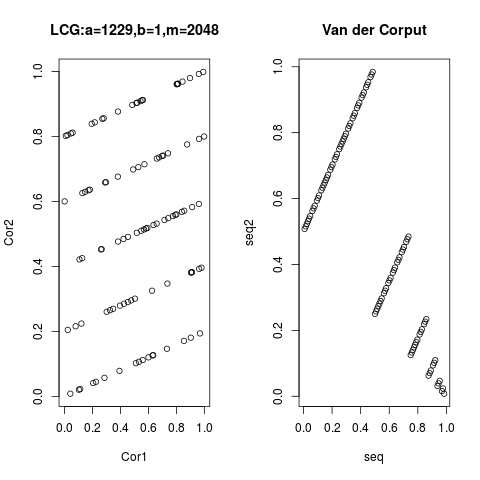
\includegraphics{Question1_5.png}
\end{center}

\newpage
\textbf{\large Question 1(f):}
The Code to implement this Question is as follows:\\

\noindent{R Code}

\lstset {language=R}


\begin{lstlisting}

a <- 1229;
b <- 1;
m <- 2048;
x <- 0;
x <- (a*x+b)%%m;
u <- x/m;
Cor1=NULL;
Cor2=NULL;

for(i in 1:100000)
{
	x <- (a*x+b)%%m;
	Cor1[i]=u;
	u <- x/m;
	Cor2[i] <- u;
}


seq=NULL;
for(i in 1:100001){
	p=NULL;
	res <- 0;
	num=i;
	for(j in 1:18){
		p[j]=num%%2;
		num=num%/%2;
	}
	for(k in 1:18){
		res=res+p[k]*2^(-k);
	}
	seq[i]=res;
}
#Making 2-D pairs.
seq2=NULL;
for(s in 1:100000){
	seq2[s]=seq[s+1];
}
length(seq) <- 100000;

pk=c(0,1);

old.par <- par(mfrow=c(1, 2));
plot(Cor1, Cor2, main="LCG:a=1229,b=1,m=2048");
plot(seq, seq2,  main="Van der Corput");
par(old.par);


\end{lstlisting}


\begin{center}
	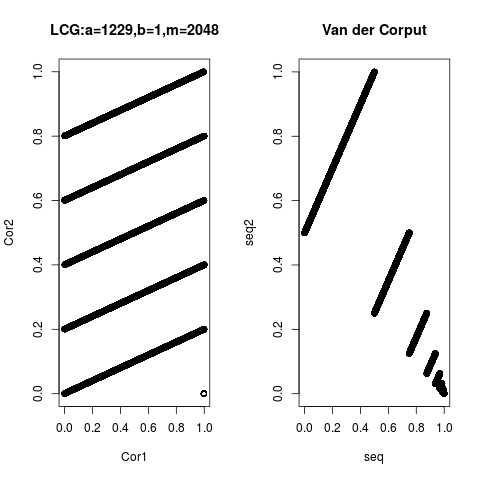
\includegraphics{Question1_6.png}
\end{center}
\newpage
\textbf{\large Question 2(a):}
The Code to implement this Question is as follows:\\

\noindent{R Code}

\lstset {language=R}


\begin{lstlisting}

seq=NULL;
for(i in 1:100){
	p=NULL;
	res <- 0;
	num=i;
	for(j in 1:8){
		p[j]=num%%2;
		num=num%/%2;
	}
	for(k in 1:8){
		res=res+p[k]*2^(-k);
	}
	seq[i]=res;
}
seq2=NULL;
for(i in 1:100){
	p=NULL;
	res <- 0;
	num=i;
	for(j in 1:5){
		p[j]=num%%3;
		num=num%/%3;
	}
	for(k in 1:5){
		res=res+p[k]*3^(-k);
	}
	seq2[i]=res;
}
plot(seq,seq2);


\end{lstlisting}


\begin{center}
	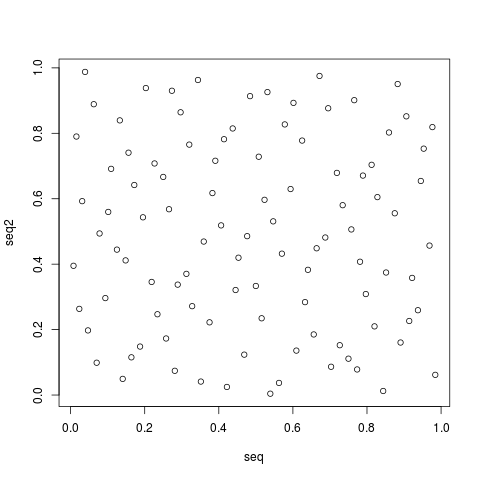
\includegraphics{Question2_1.png}
\end{center}
\newpage
\textbf{\large Question 2(b):}
The Code to implement this Question is as follows:\\

\noindent{R Code}

\lstset {language=R}


\begin{lstlisting}

seq=NULL;
for(i in 1:100000){
	p=NULL;
	res <- 0;
	num=i;
	for(j in 1:18){
		p[j]=num%%2;
		num=num%/%2;
	}
	for(k in 1:18){
		res=res+p[k]*2^(-k);
	}
	seq[i]=res;
}
seq2=NULL;
for(i in 1:100000){
	p=NULL;
	res <- 0;
	num=i;
	for(j in 1:11){
		p[j]=num%%3;
		num=num%/%3;
	}
	for(k in 1:11){
		res=res+p[k]*3^(-k);
	}
	seq2[i]=res;
}
plot(seq,seq2);


\end{lstlisting}


\begin{center}
	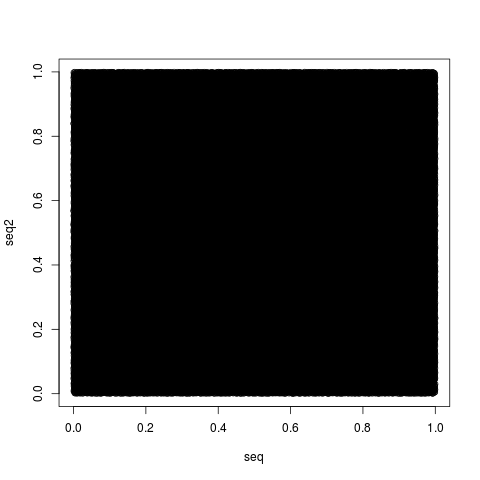
\includegraphics{Question2_2.png}
\end{center}

We observe that Halton Sequence is uniformly distributed in the Real plane. The Generated sequence of 2-tuples are uniformly distributed all throughout [0,1]x[0,1].








\end{document}